\documentclass[12pt]{article}

% set indentation
\usepackage{parskip}
%\setlength{\parindent}{16mm}

% for the figures
\usepackage{graphicx}
\usepackage{extsizes}
\usepackage{wrapfig}
\usepackage{leftidx}
% change margins
\usepackage{geometry}
\geometry{left=20mm,right=20mm,top=15mm,bottom=15mm}

% for the reference
\usepackage[sort]{natbib}
\usepackage{url}
\usepackage{placeins}
%\usepackage{authblk}
\usepackage{setspace}
\usepackage{tabularx}
%\doublespacing
% in preamble
%\usepackage{movie15}
% in documenet

\usepackage{authblk}
\usepackage{graphicx}
\usepackage{mathptmx} 
% My packages
\usepackage{parskip}
\usepackage{relsize, threeparttable}
\usepackage{array}
\usepackage{booktabs}
\usepackage{lscape}
\usepackage{tabularx}
\usepackage{makecell}
\usepackage{booktabs}
\usepackage{numprint}
\usepackage{amsmath}
\usepackage{mathtools}
\usepackage{amssymb}
\usepackage{multirow}
\setlength{\parindent}{16mm}
% for the figures
\usepackage{graphicx}
\usepackage{placeins}
% for the reference
\usepackage{natbib}
\usepackage{floatrow}
\usepackage{chngcntr}
\usepackage{url}
\usepackage{dutchcal}
%\usepackage{boondox-calo}
\usepackage{upgreek}
%\date{}
\usepackage{color,soul}
\usepackage{amsmath}

\setlength{\parindent}{0pt}
\definecolor{lightgrey}{rgb}{0.925, 0.925, 0.925}
\sethlcolor{lightgrey}







\title{Unraveling the time dynamics of life annuities}

\author[1]{Jes\'us-Adri\'an \'Alvarez\thanks{jeal@atp.dk}}

\author[2]{Andr\'es M. Villegas}

\affil[1]{{\small Danish Labour Market Supplementary Pension Fund (ATP), Kongens V\ae nge 8, 3400 Hiller\o d, Denmark} }

\affil[2]{\small{School of Risk and Actuarial Studies and ARC Centre of Excellence in Population Ageing Research (CEPAR)\\ UNSW Business School, Sydney, Australia}}
%\date{}

\begin{document}
\maketitle

{
\setcounter{tocdepth}{2}
%\tableofcontents
}



\begin{abstract}
	
	POLISH THE ABSTRACT
	Actuaries and risk managers are interested in developing strategies to ensure that changes in interest rates do not affect the value of a portfolio. Similarly, there is a long-standing tradition among demographers to measure how changes over time in mortality affect summary measures of longevity such as life expectancy. In this paper, we bring these two perspectives together. We develop a new decomposition method to quantify the contribution of changes in mortality and interest rates to the change in life annuity factors. We introduce neat and intuitive formulations that allow actuaries and risk managers to easily asses stochastic changes in financial and longevity risks embedded in their life annuities' portfolios. \\
	
	To illustrate our method, we look at the long-term development of life annuity prices using financial and mortality data from the United Kingdom since 1841. We found that there is clear interplay between longevity and financial risk, where the former one is at times masked by high financial risk. 
\end{abstract}
\newpage
\section{Introduction}\label{sec:1_introduction}

There is a prevalent concern among pension funds and insurance companies about how simultaneous fluctuations in interest and mortality affect their life annuity portfolios. This concern is emphasized under the current setting that high-income countries are facing: rapid changes in interest rates, and mortality improvements \citep{djeundje2022slowdown} that have been reversed by the Covid-19 epidemic \citep{aburto2022quantifying}. There are two fundamental uncertainties about the time dynamics of life annuities. First, there is uncertainty about the development of cohort mortality and interest rates themselves. The second uncertainty relates to the sensitivity of life annuities (and corresponding reserves, capital charges, etc.) to the simultaneous change in mortality and interest rates. In other words, how mortality and interest change over time and how life annuities react to them.

The first source of uncertainty has been studied extensively and a wide range of models to forecast mortality and interest rates have been proposed under many different perspectives\footnote{It is important to highlight that forecasting (both for mortality and interest rates) is out of the scope of this paper. Instead, the focus is on the development of mathematical expressions to determine the sources of change in life annuities.} \citep{cairns2017modelling,cairns2019modelling,kallestrup2020insight} (ADD REFERENCES TO MORTALITY MODELS). The second source of uncertainty has been examined to a lesser extend. Most of the studies regarding interest-rate sensitivity are related to immunization theory, while for mortality, there is a limited number of studies that have addressed this issue. An important contribution in this regard is recently done by \citet{rabitti2020mortality}. They used model life tables for the United States in 1990 and for the United Kingdom (years 1990-1994) and assumed different levels of constant interest rates to show that, for these life tables, the sensitivity to mortality is higher when interest rate is low (i.e. 0.5\%), whereas the financial component becomes the key risk driven when both sensitives are taken into account. 


The analysis of \citet{rabitti2020mortality} makes strides in providing a joint perspective of the sensitivities to changes in mortality and interest rates. However, it is unclear whether their results hold for different time periods or with real data for the term-structure of interest rates\footnote{Specifically, because their analysis is limited to historical life tables from 30 years ago (i.e. US 1990 and the UK 1990-1994) and with the synthetic assumption of constant interest rates.}. It is also unclear how rapid the sensitives change over time and what are the sources of such changes (e.g. driving causes of death). Furthermore, differences in age-specific mortality improvements and differentials in term-specific attributions terms of the yield curve might produce contrasting effects in life annuities. At present, there is no single tool to disentangle the effect of i) simultaneous fluctuations in mortality and interest, and ii) the sensitivity to such fluctuations in life annuities, reserves and related risk measures. 

In this article, we introduce continuous-time formulations to address this issue. We quantify the simultaneous contribution of changes in mortality and interest to changes over time in life annuities. To illustrate our equations, we first look at the long-term development of life annuity factors using financial and demographic data from the United Kingdom from 1841 to 2016. Next, we dig into age-specific and term-specific attributions and ravel out the causes of death that drive the longevity component. Finally, we extend our equations to changes in reserves and develop the intuition about how such equations can be used in stochastic risk management. Our formulations are neat, intuitive and can be easily used by actuaries and risk managers to assess the financial and longevity risks embedded in their life annuities' portfolios (using their own, real data). From the actuarial perspective, our formulations are useful in devising strategies for better risk management by levering on well-known results from mathematical demography and immunization.


We have organized the remainder of the article as follows. First, we describe useful results from the actuarial and demographic literature on mortality and interest rate sensitivities in Section \ref{sec:2_Sensitivity}. Next, we derive the equations to unravel the sources of changes over time in life annuities in Section \ref{sec:3_timedynamics}. Then, in Section \ref{sec:4_Illustration}, we illustrate our equations with historical data from the United Kingdom. In Section \ref{sec:5_Reserves}, we extend our equations to annuity reserves and risk management. Lastly, we conclude with a discussion about the applicability of the equations developed in this paper. The code to replicate the results and all the deriviations introduced in this article are available in the following open-source repository: \textit{link available upon publication}.



\section{Sensitivity to interest and mortality changes}\label{sec:2_Sensitivity}

\textit{\textbf{Duration}}

 Duration (hereafter denoted by $D$) is a fundamental quantity used to measure the effect of interest rates in any financial instrument. It is defined as the price sensitivity of a life annuity (or bond, fixed income, or any other financial instrument) to changes in the force of interest $\delta$ \citep{milevsky2013life,charupat2016sluggish}. There are different types of duration and according to their interpretation, they can be used in different applications. For example, Macaulay duration estimates how many years it will take for an investor to be repaid the bond's price by its total cash flows. Modified duration measures the price change in a bond given a 1\% change in interest rates. Mathematically, duration is the first-order derivative of the financial quantity with respect to $\delta$, whereas the second-order derivative is given by the convexity. Both, duration and convexity are used in interest-rate immunization \citep{redington1951papers,fisher1971coping,shiu1990redington,santomero1997financial,courtois2007immunization} where portfolios are hedged against fluctuations in interest rates.


\textit{\textbf{Entropy}}


The entropy (hereafter denoted by $H$) is a measure developed by demographers and population biologists to quantify the sensitivity of life expectancy to changes in the force of mortality \citep{leser1955variations,keyfitz1977difference,demetrius1974demographic,goldman1986new,Vaupel1986}, such that higher the values of the entropy; the higher the sensitivity of life expectancy is to mortality rates. It has been shown that the entropy increases or decreases depending of the ages where mortality improvements take place \citep{aburto2019threshold}. The entropy is also been used by demographers as an indicator of how lifespans vary within populations \citep{vaupel2011life,fernandez2015entropy,aburto2020dynamics}.

An important contribution in understanding the time dynamics of life expectancy via the entropy is done by \citet{Vaupel2003}. They show that the time derivative of life expectancy ($e(0,t)$) with respect to time $t$ can be expressed in terms of the general pace of mortality improvement ($\rho_{e}$) and the entropy ($H_{e}(t)$), such that:

\begin{equation}\label{eq:lifeexpdecomp}
	\dfrac{\partial e(0,t)}{\partial t}= \rho_{e}(t)H_{e}(t)e(0,t).
\end{equation}


Equation (\ref{eq:lifeexpdecomp}) clearly disentangles the changes over time in mortality and the sensitivity of life expectancy to these changes. This Equation allows further decomposition of age-specific and cause-specific contributions to mortality improvement and entropy.

\citet{Haberman2011} extended the concept of entropy to life annuities. In this context, the entropy measures the sensitivity of a life annuity to proportional changes in the force of mortality. The entropy of can be seen as an indicator longevity risk \citep{rabitti2020mortality}. \citet{alvarez2021linking} shows that it can be used to examine socio-economic disparities in pension systems.

There is a growing line of research that has used the entropy\footnote{with the name of mortality durations but it is essentially the same formulation as in \citet{Haberman2011}} in the context of mortality-immunization\footnote{similar to interest-immunization, mortality-immunization is defined as a set of strategies to ensure that the value of a portfolio will be little affected in response to changes in mortality rates}. In particular, \citet{wang2010optimal,tsai2011actuarial,Tsai2013a,Li2011} derive discrete formulas for life annuity entropies and convexities assuming constant and proportional changes in the force of mortality, $\mu$. Mortality-immunization has been applied to different types of life insurance and annuity products \citep{li2012key,Li2012,Wong2015,Luciano2015,levantesi2018natural}. 

\textit{\textbf{Bringing both perspectives together}}

Research regarding the sensitivity to mortality changes (mostly developed by demographers) and on sensitivity to interest rates (mostly developed by actuaries and financial managers) have remained largely disconnected\footnote{with exception of \citet{Haberman2011,rabitti2020mortality,alvarez2021linking} that made clear the links between both strands of research}. Paradoxically, both strands of research direct efforts at the same objective of study: gain a better understanding of the inherent sources of change in life contingent quantities.

Recently, \citet{Lin2020} made strides on this regard by deriving discrete formulas to calculate sensitivity of life annuities (and whole life insurances) to simultaneous changes mortality and interest rates. They introduced a synthetic variable called 'the force of mortality-interest`, which results from the addition of the force of mortality and interest ($\mu^*=\mu+\delta$). While the application of \citet{Lin2020} is interesting since it combines sensitivity in mortality and interest rates, it is unlikely that $\mu$ and $\delta$ change at the same pace over time. 

In this article we bring together the aforementioned results from the actuarial and demographic literature to the analysis of the time dynamics of life annuities. In the following section, we derive equations to this aim and describe their applications.

\section{Time dynamics of life annuities}\label{sec:3_timedynamics}
\subsection{Preliminaries}\label{preliminaries}

All of the quantities introduced in this section vary over time $t$. Following the standard actuarial notation, we define the following quantities:

\begin{itemize}

\item
\(\mu(x,t)\) is the force of mortality at age \(x\) in time $t$.

\item
$_sp_x(t)=e^{-\int_{0}^{s}\mu(x+y,t)dy}$ is the time $t$ period survival probability from age \(x\) to age \(x+s\). 


\item
\(\delta(s,t)\) is the time $t$ forward force of interest at maturity $s$. This measure is a general form to express the term-structure of interest rates.

\item 

${v}(s,t)=e^{-\int_{0}^{s}\delta(y,t)dy}$ is the time $t$ discount factor, for a cash-flow payable at maturity $s$.

\end{itemize}

The derivative with respect to time $t$ is denoted by adding a point on top of the function of interest. For example, time derivatives for the forces of mortality and interest are expressed as:

\begin{equation} \label{eq:mudot}
\dot{\mu}(x,t)\equiv\frac{\partial\mu(x,t)}{\partial t},
\end{equation}

and 

\begin{equation} \label{eq:mudot}
\dot{\delta}(s,t)\equiv\frac{\partial\delta(s,t)}{\partial t}.
\end{equation}

The rate of mortality improvement (or progress in reducing mortality) at age \(x\) is defined as

\begin{equation} \label{eq:rho}
\rho(x,t)=-\frac{\frac{\mu(x,t)}{\partial t}}{\mu(x,t)} = - \frac{\dot{\mu}(x,t)}{\mu(x,t)}.
\end{equation}

Similarly, the relative change over time in the force of interest at maturity $s$ is captured by 

\begin{equation} \label{eq:phi}
\upvarphi(s,t)=-\frac{\frac{\delta(s,t)}{\partial t}}{\delta(s,t)} = -\frac{\dot{\delta}(s,t)}{\delta(s,t)}.
\end{equation}

The actuarial present value of a continuous life annuity at age $x$ evaluated at time $t$ is given by

\begin{equation}\label{eq:Annuity}
\bar{a}_x(t) = \int_0^\infty {}_sp_x(t) {v}(s,t)ds = \int_0^\infty {}_sE_x(t) ds,
\end{equation}

where ${}_sE_x(t)={}_sp_x(t) {v}(s,t)$. 

A life annuity deferred $s$ years starting to be paid at age $x+s$ is expressed as

\begin{equation}\label{eq:DefAnnuity}
{}_s|\bar{a}_x(t) = {}_sE_x(t) \bar{a}_{x+s}(t).
\end{equation}


\subsection{Two types of changes: constant and proportional to $\mu$ and $\delta$}


We are interested in measuring changes in $\bar{a}_x(t)$ with respect to the time variable $t$. To achieve this aim, we first need to describe how $\bar{a}_x(t)$ reacts to changes in the forces of mortality and interest. As mentioned in Section \ref{sec:2_Sensitivity}, the entropy of a life annuity as the measure that captures changes in $\bar{a}_x(t)$ with respect to $\mu(x,t)$. Formally, it is defined as 

\begin{equation}\label{eq:EntropyGeneral}
{H}_{x}(t) = \frac{ \frac{\partial \bar{a}_x(t) }{\partial \mu(x,t)}}{\bar{a}_x(t)}.
\end{equation}

Analogously, duration captures the sensitivity of $\bar{a}_x(t)$ to changes in interest rates. It is defined as the relative derivative of the annuity factor with respect to changes in the force of interest \citep{Milevsky2012,Milevsky2012a}:


\begin{equation}\label{eq:DurationGeneral}
{D}_{x}(t) = \frac{ \frac{\partial \bar{a}_x(t) }{\partial \delta(s,t)}}{\bar{a}_x(t)}.
\end{equation}

Greater values for ${H}_{x}(t)$ and ${D}_{x}(t)$ indicate that $\bar{a}_x(t)$ is highly sensitive to changes in $\mu(x,t)$ and $\delta(s,t)$ respectively. The entropy and the duration of a life annuity can be measured either by assuming constant or proportional changes in $\mu(x,t)$ and $\delta(s,t)$. All formulations in the following sections are developed for both cases. 



\textit{\textbf{{Changes in $\bar{a}_x(t)$ with respect to $\mu(x,t)$}}}

The entropy of a life annuity is denoted by ${H}^{c}_{x}(t)$ when changes in $\mu(x,t)$ are held constant at all ages and by ${H}^{p}_{x}(t)$ when changes are performed proportional. Based on the results developed by \citet{Tsai2013a} and \citet{Lin2020}, when $\mu(x,t)$ is changed constantly to $\mu(x,t)+\gamma$ such that $\gamma$ is a small number (see proof in the Appendix), the entropy of $\bar{a}_x(t)$ becomes

\begin{equation}\label{eq:EntropyC}
{H}^{c}_{x}(t) = -\frac{\int_{0}^\infty s {}_sp_x(t) {v}(s,t) ds}{\bar{a}_x(t)}=\frac{{h}^{c}_{x}(t)}{\bar{a}_x(t)},
\end{equation}

where ${h}^{c}_{x}(t)=-\int_{0}^\infty s {}_sp_x(t) {v}(s,t) ds$. The term ${h}^{c}_{x}(t)$ is expressed in absolute (monetary) terms, whereas the entropy ${H}^{c}_{x}(t)$ is dimensionless because it does not depend on the absolute value of $\bar{a}_x(t)$.


\citet{Haberman2011} and \citet{Tsai2013a} show that when changes in $\mu(x,t)$ are assumed to be proportional to a small number $\gamma$ such that $\mu(x,t)(1+\gamma)$, the entropy of $\bar{a}_x(t)$ becomes

\begin{equation} \label{eq:EntropyP}
{H}^{p}_{x}(t) = -\frac{ \int_{0}^{\infty}{}_sp_x(t)\ln[{}_sp_x(t)] {v}(s,t) ds}{\int_0^\infty {}_sp_x(t) {v}(s,t) ds}.
\end{equation}


Alternatively, we show (see proof in Section \ref{sec:EntropyAlt} of the Appendix) that Equation (\ref{eq:EntropyP}) can be expressed as

\begin{equation} \label{eq:EntropyP2}
\begin{split}
{H}^{p}_{x}(t) &=  \frac{\int_0^\infty \mu(x+s,t)   {}_s|\bar{a}_x(t) ds}{\bar{a}_x(t)} =  \frac{{h}^{p}_{x}(t)}{\bar{a}_x(t)}, 
\end{split}
\end{equation}

where ${h}^{p}_{x}(t)=\int_0^\infty \mu(x+s,t)   {}_s|\bar{a}_x(t) ds$. Analogous to the case where changes are assumed to be constant, quantities ${h}^{p}_{x}(t)$ and ${H}^{p}_{x}(t)$ are expressed in absolute and relative terms respectively. The formulations shown in this section are closely related to the ones developed in the mortality-immunization literature \citep{Tsai2013a,Lin2020}. We extended them to the continuous case.

 
 

\textbf{\textit{{Changes in $\bar{a}_x(t)$ with respect to $\delta(s,t)$}}}

 Similar to the entropy, changes in $\bar{a}_x(t)$ with respect to $\delta(s,t)$ can be assumed to be either constant or proportional. Duration assuming constant changes in $\delta(s,t)$ is denoted by ${D}^{c}_{x}(t)$, whereas ${D}^{p}_{x}(t)$ refers to the duration assuming proportional changes. For the former case we have that:



\begin{equation}\label{eq:DurationC}
\begin{split}
{D}^{c}_x(t)&= -\frac{\int_0^\infty s {}_sp_x(t) {v}(s,t)ds}{\bar{a}_x(t)} \\
&= \frac{{d}^{c}_x(t)}{\bar{a}_x(t)},
\end{split}
\end{equation}

where ${d}^{c}_x(t)=-\int_0^\infty s {}_sp_x(t) {v}(s,t)ds$. Thus, assuming constant changes in $\delta(s,t)$ results into common types of duration known in finance as \textit{dollar duration}, ${d}^{c}_x(t)$, and \textit{modified duration}, ${D}^{c}_x(t)$ (see \citet{Milevsky2012} and \citet{Tsai2013a} for further details). It is worth noting that Equations (\ref{eq:EntropyC}) and (\ref{eq:DurationC}) are identical such that ${d}^{c}_x(t)={h}^{c}_{x}(t)$. Interestingly, this indicates that constant (i.e. parallel) changes in the force of mortality have essentially the same effect as parallel changes in the force of interest.


Assuming proportional changes in $\delta(s,t)$ (see proof in the Appendix) results in: 


\begin{equation}\label{eq:DurationP}
\begin{split}
{D}^{p}_{x}(t) &= -\frac{\int_0^\infty {}_sp_x(t) v(s,t) \ln(v(s,t))ds}{\bar{a}_x(t)}. \\
\end{split}
\end{equation}


Note that when assuming constant force of mortality such that $v(s,t)=e^{-\delta(t)s}$, we have that ${D}^{p}_{x}(t)=\delta(t){D}^{c}_{x}(t)$,


\begin{equation}\label{eq:DurationCP}
\begin{split}
{D}^{p}_{x}(t) &= -\frac{\int_0^\infty {}_sp_x(t) v(s,t) \ln(v(s,t))ds}  {\bar{a}_x(t)} \\
&=- \delta(t)\frac{\int_0^\infty s{}_sp_x(t) e^{-\delta(t)s}  ds}{\bar{a}_x(t)} \\
& = \delta(t){D}^{c}_{x}(t).
\end{split}
\end{equation}

Equation (\ref{eq:DurationP}) can also be re-expressed as:

\begin{equation}\label{eq:DurationP2}
\begin{split}
{D}^{p}_{x}(t) &= \frac{\int_0^\infty \delta(s,t) {}_s|\bar{a}_x(t)ds} {\bar{a}_x(t)} \\
                 &= \frac{{d}^{p}_{x}(t)}{\bar{a}_x(t)}.
\end{split}
\end{equation}


where ${d}^{p}_{x}(t)=\int_0^\infty \delta(s,t) {}_s|\bar{a}_x(t) ds$. 




\subsection{Time derivative of $\bar{a}_x(t)$} \label{sec:timderiv}

We now compute the derivative of $\bar{a}_x(t)$ with respect to the time variable $t$, $\dot{\bar{a}} _x(t)=\frac{\partial \bar{a}_x(t)}{\partial t}$, such that

\begin{equation}\label{eq:TimeDeriv}
\begin{split}
\dot{\bar{a}} _x(t) &= \int_0^\infty {}_s\dot{p}_x(t) v(s,t)ds +\int_0^\infty {}_sp_x(t) \dot{v}(s,t)ds.\\
\end{split}
\end{equation}


To develop a closed-form solution for Equation (\ref{eq:TimeDeriv}) we consider the general case where $_sp_x(t)=e^{-\int_{0}^{s}\mu(x+y,t)dy}$ and ${v}(s,t)=e^{-\int_{0}^{s}\delta(s,t)dy}$. We analyse separately each of the two terms in the right side of Equation (\ref{eq:TimeDeriv}). Let us first focus on the first term:


\begin{equation}\label{eq:TimeDerivP1}
\begin{split}
\int_0^\infty {}_s\dot{p}_x(t) v(s,t)ds &= \int_0^\infty   v(s,t) e^{-\int_0^{s}\dot{\mu}(x+y,t)dy}ds\\
&= -\int_0^\infty   v(s,t) {}_sp_x(t)\int_0^{s}\dot{\mu}(x+y,t)dyds\\
&= -\int_0^\infty  \dot{\mu}(x+s,t) \int_s^{\infty} v(y,t) {}_yp_x(t) dyds\\
&= - \int_0^\infty \dot{\mu}(x+s,t)   {}_sE_x(t) \bar{a} _{x+s}(t) ds\\
&= \int_0^\infty \rho(x+s,t) \mu(x+s,t)   {}_s|\bar{a}_x(t) ds.\\
\end{split}
\end{equation}


The second part equals:

\begin{equation}\label{eq:TimeDerivP2}
\begin{split}
\int_0^\infty {}_sp_x(t) \dot{v}(s,t)ds &= \int_0^\infty {}_sp_x(t)  e^{-\int_0^{s}\dot{\delta}(y,t)dy}ds\\
&= -\int_0^\infty {}_sp_x(t) v(s,t) \int_0^{s}\dot{\delta}(y,t)dy ds\\
&= -\int_0^\infty  \dot{\delta}(s,t)\int_s^{\infty} {}_yp_x(t) v(y,t) dy ds\\
&= \int_0^\infty  \upvarphi(s,t) \delta(s,t)  {}_s|\bar{a}_x(t) ds.\\
\end{split}
\end{equation}


Thus, $\dot{\bar{a}} _x(t)$ can be expressed as


\begin{equation}\label{eq:TimeDerivP3}
\begin{split}
\dot{\bar{a}}_{x}(t) &=  \int_0^\infty \rho(x+s,t) \mu(x+s,t){}_s|\bar{a}_x(t) ds +\int_0^\infty  \upvarphi(s,t) \delta(s,t)  {}_s|\bar{a}_x(t) ds\\
&= \int_0^\infty \rho(x+s,t) {}_sM_x(t)  ds +\int_0^\infty  \upvarphi(s,t) {}_sW_x(t)  ds,
\end{split}
\end{equation}


where ${}_sM_x(t)= \mu(x+s,t){}_s|\bar{a}_x(t)$ and ${}_sW_x(t)=\delta(s,t)  {}_s|\bar{a}_x(t)$. Dividing Equation (\ref{eq:TimeDerivP3}) by $\bar{a}_x(t)$ yields to:


\begin{equation}\label{eq:TimeDerivP}
\begin{split}
 \acute{\bar{a}}_x(t) = \frac{\dot{\bar{a}}_x(t)}{\bar{a}_x(t)}  = 
 \underbrace{\bar{\rho}_x(t){H}^{p}_x(t)}_\text{longevity component}
 +\underbrace{\bar{\upvarphi}(t){D}^{p}_x(t),}_\text{financial component}
\end{split}
\end{equation}

where $\bar{\rho}_x(t)= \frac{\int_0^\infty \rho(x+s,t) {}_sM_x(t)  ds}{\int_0^\infty  {}_sM_x(t)ds}$ and 
$\bar{\upvarphi}(t)= \frac{\int_0^\infty \upvarphi(s,t) {}_sW_x(t)  ds}{\int_0^\infty {}_sW_x(t) ds}$ are the weighted average paces of change in mortality and interest rates respectively. Functions $\bar{\rho}_x(t)$ and $\bar{\upvarphi}(t)$ capture the stochastic change in the forces of mortality and interest whereas ${H}^{p}_x(t)$ and ${D}^{p}_x(t)$ capture the sensitivity due to changes in $\mu$ and $\delta$. In other words, Equation (\ref{eq:TimeDerivP}) entails that changes over time in annuity factors are driven by $\bar{\rho}_x(t)$ and $\bar{\upvarphi}(t)$, which are modulated by ${H}^{p}_x(t)$ and ${D}^{p}_x(t)$ respectively\footnote{Equation (\ref{eq:TimeDerivP}) can be seen as an extension of the Equation (\ref{eq:lifeexpdecomp}) developed by \citet{Vaupel2003} to measure changes over time in life expectancy}.


\subsection{Age and term contributions to changes in $\bar{a}_x(t)$}

Equation (\ref{eq:TimeDerivP}) gives a general way of understanding the sensitivity of the value of an annuity to overall changes in mortality and the term structure of interest rates. However, we may also be interested in understanding the contribution of particular age groups or specific terms of the yield curve to changes in the life annuity portfolio. This is in the spirit of the perfomance attribution exercises that are common in fixed income (see, e.g., \citet{Daul2012}).

 Let us define $n$ age groups $[x_{i-1}, x_i)$, $i=1,\ldots,n$, with $x_0=x$ and $x_n=\infty$, and $m$ term groups $[t_{j-1}, t_j)$, $j=1,\ldots,m$, with $t_0=0$ and $t_m=\infty$. Equation (\ref{eq:TimeDerivP3}) can be decomposed by age and term groups as follows:

\begin{equation}\label{eq:TimeDerivAge}
\begin{split}
 \acute{\bar{a}}_x(t) = \sum_{i=1}^n\int_{x_{i-1}-x}^{x_i-x}  \rho(x+s,t) {}_sM_x(t)  ds +\sum_{j=1}^m\int_{t_{j-1}}^{t_j}   \upvarphi(s,t) {}_sW_x(t)  ds.  
\end{split}
\end{equation}
We can also decompose the entropy $h_x^p(t)$ into $n$ age groups as follows:

\begin{equation} \label{eq:EntropyAge}
\begin{split}
{h}^{p}_{x}(t) &=  \sum_{i=1}^n\int_{x_{i-1}-x}^{x_i-x} \mu(x+s,t)   {}_s|\bar{a}_x(t) ds \\
&=  \sum_{i=1}^n {h}^{p}_{x}(t;x_{i_1},x_{i}),
\end{split}
\end{equation}
with ${h}^{p}_{x}(t;x_{i-1},x_{i})=\int_{x_{i-1}-x}^{x_i-x} \mu(x+s,t)   {}_s|\bar{a}_x(t) ds$, denoting the dollar entropy associated to proportional changes in the force of mortality between ages $x_{i-1}$ and $x_{i}$ and ${H}^{p}_{x}(t;x_{i-1},x_{i}) = \frac{{h}^{p}_{x}(t;x_{i-1},x_{i})}{\bar{a}_x(t)}$, the corresponding dimensionless entropy. 

Similarly, we can decompose the dollar duration $d^p(t)$ into $m$ term groups as follows:

\begin{equation}\label{eq:DurationAge}
\begin{split}
{d}^{p}_{x}(t) &= \sum_{j=1}^m\int_{t_{j-1}}^{t_j} \delta(s,t) {}_s|\bar{a}_x(t)ds \\
&= \sum_{j=1}^m {d}^{p}_{x}(t;t_{j-1},t_{j}),
\end{split}
\end{equation}

with ${d}^{p}_{x}(t;t_{j-1},t_{j}) = \int_{t_{j-1}}^{t_j} \delta(s,t) {}_s|\bar{a}_x(t)ds$, denoting the dollar duration associated to proportional changes in term structure between terms $t_{j-1}$ and $t_{j}$ and ${D}^{p}_{x}(t;t_{j-1},t_{j}) = \frac{{d}^{p}_{x}(t;t_{j-1},t_{j})}{\bar{a}_x(t)}$, the corresponding dimensionless duration. These age-specific entropies and term-specific durations are akin to the key q-durations \citep{li2012key} and key rate durations \citep{Ho1992}, which measure the sensitivity of financial instruments to changes in specific portions of the life table and term structure of interest rates.\\

Combining Equations (\ref{eq:TimeDerivAge}), (\ref{eq:EntropyAge}), (\ref{eq:DurationAge}):  

\begin{equation}\label{eq:TimeDerivAge2}
\begin{split}
 \acute{\bar{a}}_x(t) = \sum_{i=1}^n\bar{\rho}_x(t;x_{i-1}, x_i){H}^{p}_x(t;x_{i-1}, x_i) +\sum_{j=1}^m\bar{\upvarphi}(t;t_{j-1},t_{j}){D}^{p}_x(t;t_{j-1},t_{j}),  
\end{split}
\end{equation}
where $$\bar{\rho}_x(t;x_{i-1}, x_i)= \frac{\int_{x_{i-1}-x}^{x_i-x} \rho(x+s,t) {}_sM_x(t)  ds}{\int_{x_{i-1}-x}^{x_i-x}  {}_sM_x(t)ds}$$ and 
$$\bar{\upvarphi}(t;t_{j-1},t_{j})= \frac{\int_{t_{j-1}}^{t_{j}} \upvarphi(s,t) {}_sW_x(t)  ds}{\int_{t_{j-1}}^{t_{j}} {}_sW_x(t) ds}$$ are, respectively, the weighted average improvement rates in the age group $[x_{i-1},x_{i})$ and the weighted average pace of change in the force of interest for the term group $[t_{j-1},t_{j})$. 





\subsection{Cause of death decomposition}

Depending on the population, different causes of death can contribute substantially to the dynamics of the life annuity portfolio \citep{lin2005securitization,kallestrup2020insight}. A contemporary issue related to this pattern is the case of the excess mortality due to Covid-19 observed worldwide during the years 2020 and 2021 \citep{aburto2022quantifying}. To get insights about how causes of death shape the time dynamics of life annuities, the longevity component of Equation (\ref{eq:TimeDerivP}) can be easily decomposed into cause-specific contributions. 

Let ${_s}p{^i_x}(t)=e^{-\int_{0}^{s}\mu{^i}(x+y,t)dy}$ be the probability of surviving cause $i$ from age \(x\) to age \(x+s\) at time $t$, and $\mu{^i}(x+y,t)$ be the associated hazard. For $i=1,\dots,n$ independent causes of death, we have that ${_s}p{_x}(t)= \prod_{i=1}^{n} {_s}p{^i_x}(t)$. In this context, a whole life annuity can be expressed as $\bar{a}_x(t) = \int_0^\infty {_s}p{^1_x}(t) \cdots{_s}p{^n_x}(t) {v}(s,t)ds$. Deriving $\bar{a}_x(t)$ with respect to time $t$ yields to


\begin{equation}\label{eq:TimeDerivCoD}
\begin{split}
\dot{\bar{a}} _x(t) &= \int_0^\infty   {_s}\dot{p}{^1_x}(t) \cdots{_s}p{^n_x}(t) v(s,t)ds +\dots+\int_0^\infty   {_s}{p}{^1_x}(t) \cdots{_s}\dot{p}{^n_x}(t) v(s,t)ds +
\int_0^\infty {}_sp_x(t) \dot{v}(s,t)ds\\
&= \int_0^\infty  {_s}\acute{p}{^1_x}(t)  {_s}{p}{^1_x}(t) \cdots{_s}p{^n_x}(t) v(s,t)ds +\dots+\int_0^\infty   {_s}{p}{^1_x}(t) \cdots{_s}\acute{p}{^n_x}(t){_s}{p}{^n_x}(t) v(s,t)ds +\int_0^\infty {}_sp_x(t) \dot{v}(s,t)ds\\
&= \int_0^\infty  {_s}\acute{p}{^1_x}(t)  {_s}{p}{_x}(t)v(s,t)ds +\dots+\int_0^\infty   {}_s\acute{p}{^n_x}(t) {_s}{p}{_x}(t) v(s,t)ds +\int_0^\infty {}_sp_x(t) \dot{v}(s,t)ds\\
&= \sum_{i=1}^{n} \int_0^\infty  {_s}\acute{p}{^i_x}(t)  {_s}{p}{_x}(t)v(s,t)ds +\int_0^\infty {}_sp_x(t) \dot{v}(s,t)ds.
\end{split}
\end{equation}


Following the same procedure of Equation (\ref{eq:TimeDerivP1}), each component $\int_0^\infty  {_s}\acute{p}{^i_x}(t)  {_s}{p}{_x}(t)v(s,t)ds$ reduces to $\int_0^\infty  \rho^{i}(x+s,t){}_sM^{i}_x(t)ds$, where ${}_sM^{i}_x(t)= \mu^{i}(x+s,t){}_s|\bar{a}_x(t)$.  The last component of Equation (\ref{eq:TimeDerivCoD}) equals $\int_0^\infty  \upvarphi(s,t) {}_sW_x(t) ds$ as in Equation (\ref{eq:TimeDerivP3}). Thus, Equation (\ref{eq:TimeDerivCoD}) equals


\begin{equation}\label{eq:TimeDerivCoD2}
\begin{split}
\dot{\bar{a}} _x(t) &= \sum_{i=1}^{n} \int_0^\infty  \rho^{i}(x+s,t){}_sM^{i}_x(t)ds +\int_0^\infty  \upvarphi(s,t) {}_sW_x(t) ds.
\end{split}
\end{equation}

Dividing by $\bar{a} _x(t)$ we have


\begin{equation}\label{eq:TimeDerivCoD3}
\begin{split}
\acute{\bar{a}} _x(t) &= \sum_{i=1}^{n} \bar{\rho}{^i_x}(t){H}^{i}_x(t)+\bar{\upvarphi}(t){D}{^P_x}(t),
\end{split}
\end{equation}


where ${H}^{i}_x(t)=\dfrac{\int_{0}^{\infty}{}_sM^{i}_x(t)ds}{\bar{a} _x(t)}$ is the cause-specific entropy and $\bar{\rho}{^i_x}(t)=\dfrac{\int_{0}^{\infty}\rho{_x^i}(x+s,t) {}_sM^{i}_x(t)ds}{\int_{0}^{\infty}{}_sM^{i}_x(t)ds}$ is the average rate of mortality improvement of cause $i$.

\subsection{Assuming constant force of interest}


It is common that life annuities are computed by using a single interest rate, which represents the long-term expected return. Thus, $\acute{\bar{a}}_x(t)$ can be re-expressed by assuming a single interest rate $\delta(t)$ that varies over time $t$, such that $v(s,t)=e^{-\delta(t)s}$. This assumption affects the second part of Equation (\ref{eq:TimeDeriv}) as: 




\begin{equation}\label{eq:TimeDerivC1}
\begin{split}
\int_0^\infty {}_s{p}_x(t) \dot{v}(s,t)ds &=\int_0^\infty {}_s{p}_x(t) \frac{\partial \left[ e^{-\delta(t)s} \right]}{\partial t}ds \\
&=-\dot{\delta}(t)\int_0^\infty s  {}_s{p}_x(t) e^{-\delta(t)s} ds \\
&=  \dot{\delta}(t)  d^{c}_x(t).
\end{split}
\end{equation}

Substituting Equations (\ref{eq:TimeDerivP1}) and (\ref{eq:TimeDerivC1}) in Equation (\ref{eq:TimeDeriv}) results into: 


\begin{equation}\label{eq:TimeDerivC2}
\begin{split}
\acute{\bar{a}}_x(t) =  \bar{\rho}(t){H}^{p}_x(t)+\dot{\delta}(t)  D^{c}_x(t).
\end{split}
\end{equation}



Given that ${D}^{p}_{x}(t)=\delta(t){D}^{c}_{x}(t)$ (see Equation (\ref{eq:DurationCP})), it is straight-froward to show that in the case of a single interest rate, Equations (\ref{eq:TimeDerivP})  and (\ref{eq:TimeDerivC2}) are equivalent. Thus, it suffices to use the entropy (${H}^{p}_x(t)$) and the modified duration ($D^{c}_x(t)$) together with $\bar{\rho}(t)$ and $\dot{\delta}(t)$ to determine the contribution of financial and longevity risks to changes over time in life annuities.





\subsection{Recap of formulations}

Throughout Section \ref{sec:3_timedynamics}, we developed equations that can be used to determine the sources of change over time in life annuities. Overall, these equations comprise a financial component and a longevity component. Depending on the application, one can get insights about the age-specific and term-specific attribution of these components as well as cause-specific contributions. One can also make assumptions about the yield rate used in the calculations of life annuity portfolios. A summary of the equations introduced in this section is shown in the Table \ref{table:Table1}. 


\begin{table}[ht]
	\centering
	\begin{tabular}{lcc}
		\toprule
		\textbf{Description}&	\textbf{Financial component} & \textbf{Longevity component}   \\
		\hline
		\textit{General representation}&	$\bar{\upvarphi}(t){D}_x(t)$                           & $\bar{\rho}(t){H}_x(t)$ \\
		\hline
		\textit{Age-Term attributions}&	$\sum_{j=1}^m\bar{\upvarphi}(t;t_{j-1},t_{j}){D}_x(t;t_{j-1},t_{j})$                               & $\sum_{i=1}^n\bar{\rho}_x(t;x_{i-1}, x_i){H}^{p}_x(t;x_{i-1}, x_i)$ \\
		\hline
		\textit{Causes of death}&	$\bar{\upvarphi}(t){D}_x(t)$   & $\sum_{i=1}^{n} \bar{\rho}{^i_x}(t){H}^{i}_x(t)$ \\
		\hline
		\textit{Single interest rate}&	$\dot{\delta}(t){D}_x(t)$ & $\bar{\rho}(t){H}_x(t)$  \\
		\bottomrule
	\end{tabular}
	\caption{{Summary of expressions of the financial and longevity components used to determine the sources of change $\acute{a}_x(t)$}.}
	\label{table:Table1}
\end{table}



One of the main advantages of our framework is that the financial and longevity components are additive. Thus, the expressions in Table \ref{table:Table1} can be easily combined to get insights about the sources of change in $\acute{a}_x(t)$. For example, it can be the case that the actuary analysing fluctuations in the pension fund is interested in determining the term-specific contribution to the financial component as well as the causes of death that drive the longevity component. To this aim, the actuary can apply the equation $\acute{a}_x(t)=\sum_{j=1}^m\bar{\upvarphi}(t;t_{j-1},t_{j}){D}_x(t;t_{j-1},t_{j})+\sum_{i=1}^{n} \bar{\rho}{^i_x}(t){H}^{i}_x(t)$ to examine such dynamics. In the following section, we illustrate how our equations can be used using empirical data.

\section{Historical changes in life annuities in the United Kingdom}\label{sec:4_Illustration}

In this section we illustrate the formulations introduced in Section \ref{sec:3_timedynamics} by examining the sources of change in the long-term development of life annuities in the United Kingdom. We use two centuries of financial and demographic data, from 1841 to 2018. Age-specific mortality rates come from the \citep{HMD2020}, whereas long-term interest rates are represented by the yield on 2.5\% consols up to 2015, then by the yield of 20 year maturity bills (Bank of England, 2021 INSERT CITE IN .BIB FILE). We smoothed mortality and interest rates using splines \citep{green1993nonparametric,camarda2012mortalitysmooth} to obtain continuous estimates of the forces of mortality and interest respectively (Figure \ref{fig:Fig1}). Using our estimates of $\mu$ and $\delta$, we construct time series for life annuities at different ages and for both sexes. In this section we first focus on life annuity factors calculated for males at age 65, which represent a cut-off age for retirement in several populations. 


\begin{center}
	\textit{Figure 1 about here}
\end{center}




The upper panel of Figure \ref{fig:Fig2} depicts values for $\bar{a}_x(t)$ from 1841 to 2018 for males at age 65. We observe that during the second half of the 19th century and up to the decade of 1940s, $\bar{a}_{65}(t)$ remained at similar levels with small fluctuations. Thereafter, $\bar{a}_{65}(t)$ exhibited a sharp decline up to the decade of 1980s, followed by an increasing pattern that has remained until recent years. The lower panel of Figure \ref{fig:Fig2} show the relative derivative of $\bar{a}_{65}(t)$ with respect to time ($\acute{\bar{a}}_{65}(t)$). It is clear that $\acute{\bar{a}}_{65}(t)$ captures well the changes over time in life annuity; positive values indicate that $\bar{a}_{65}(t)$ goes up and negative values indicate a decrease in $\bar{a}_{65}(t)$. In the following sections we analyse the sources of change in the time trend of $\acute{\bar{a}}_{65}(t)$ by making use of the equations developed in Section \ref{sec:3_timedynamics}.

 
  \begin{center}
  	\textit{Figure 2 about here}
  \end{center}
  

\subsection{Contribution of financial and longevity components to changes in $\bar{a}_x(t)$}

As shown in the formulas developed in Section \ref{sec:3_timedynamics}, changes over time in $\bar{a}_x(t)$ can be explained in terms of longevity and financial components. Each component depends on the time fluctuations of $\mu(x,t)$ and $\delta(s,t)$ (captured by $\bar{\rho}(t)$ and $\dot{\delta}(t)$ respectively) which are modulated by the sensitivity of $\bar{a}_x(t)$ to changes in the forces of mortality and interest (entropy, ${H}^{p}_x(t)$ and modified duration, ${D}^{c}_x(t)$). Figure \ref{fig:Fig3} depicts the components responsible of fluctuations over time in $\bar{a}_x(t)$.

  \begin{center}
	\textit{Figure 3 about here}
\end{center}


The upper panel of Figure \ref{fig:Fig3} shows that between 1860 and 1940, there were some periods of mortality improvements and deterioration. However, as of the 1980s, $\bar{\rho}(t)$ increased steadily indicating an average mortality improvement between 2\% to 3\%. In recent years, $\bar{\rho}(t)$ trended downwards, which coincides with the mortality deterioration currently prevailing in the United Kingdom \citep{djeundje2022slowdown}. Regarding changes over time in the force of interest, we observe that $\dot{\delta}(t)$ has also remained at similar levels for most of the observation period with some fluctuations between 1930 and 1950. Since the 1960s, $\dot{\delta}(t)$ went up rapidly reaching the highest observed increase (of around 8\% in the decade of 1970s). Thereafter, $\dot{\delta}(t)$ declined faster and moved towards negative values entailing a decline in interest rates, which is still ongoing until recent time. Trends in $\bar{\rho}(t)$ and $\dot{\delta}(t)$ are responsible for the time trend we observe in $\bar{a}_x(t)$, which is modulated by the entropy, ${H}^{p}_x(t)$, and modifed duration, ${D}^{c}_x(t)$.


The lower panel of Figure \ref{fig:Fig3} shows that during most of the observation period, ${H}^{p}_x(t)$ was higher than ${D}^{c}_x(t)$. This indicates that $\bar{a}_x(t)$ has been more sensitive to changes in mortality than to changes in interest rates. However, these sensitivities have changed over time. The entropy show a decreasing trend that prevailed until to the 1980s. Modified duration, on the other hand, remained somewhat constant over time but as of the 1950s, it trended upwards reaching its maximum in the 1980s (of about 0.8). Thereafter, it decline again. It is worth noting that during some specific years, ${H}^{p}_x(t)$ and ${D}^{c}_x(t)$ depict the same values (i.e. in the 1960s). This means that during these years, $\bar{a}_x(t)$ was equally sensitive to changes in mortality and interest rates.




Using all the measures shown in Figure \ref{fig:Fig3}, we next calculate the contributions of financial ($\dot{\delta}(t){D}^{c}_x(t)$) and longevity risks ($\bar{\rho}(t){H}^{p}_x(t)$) to changes over time in $\bar{a}_{65}(t)$. The upper panel of Figure \ref{fig:Fig4} shows $\acute{\bar{a}}_{65}$\footnote{This is the same as Figure \ref{fig:Fig2}. We show it here so the reader can make sense of the decomposition} and the lower panel shows the financial and longevity components. Positive/negative values contribute to increase/decrease in $\bar{a}_x(t)$. From Figure \ref{fig:Fig4} it is clear that both, longevity and financial risks have played an important role in the long-term development of $\bar{a}_x(t)$. 

  \begin{center}
	\textit{Figure 4 about here}
\end{center}

We can distinguish among four periods where life annuity factors fluctuated in response to specific changes in financial and longevity risks. From 1860 to 1945, stable annuity factors modulated by  contributions of longevity and financial components to the time trend. In a second period, from 1945 to 1970, we observe decreasing annuity factors mainly driven by the financial component. Around 1970, interest rates reached the highest point, which translated into a negative contribution of the financial component. In the next period, from 1970 to 2015, the time trend changed. Annuities went up due to positive contributions of both components. In the last period, from 2015 onwards, $\bar{a}_x(t)$ continue to increase with the longevity component contributing less to the trend. This reflects the deceleration of mortality improvements occurring in the United Kingdom and many other populations \cite{djeundje2022slowdown}.
 
 \subsection{Attribution across age-groups and terms}

Next, we illustrate how the longevity and financial components in Figure \ref{fig:Fig4} can be further decomposed in age-term specific attributions. The yield curve used in this analysis was constructed using government bonds in the UK (commonly known as gilts) issued at different maturities. Data on gilts was retreived from the Bank of England (2021) and it covers the years 1970-2020.


 Figure \ref{fig:Fig5} depicts the contribution of different age groups to the longevity component (i.e. ages 65-74,75-84, 85-94, 95-104) and terms in the yield curve (i.e. years 0-9, 10-19, 20-29, 30-39) from 1970 to 2018. At first glance, Figure \ref{fig:Fig5} reveals that the major contributions comes from ages 65-74 and interest rates with terms below 20 years. 

  \begin{center}
	\textit{Figure 5 about here}
\end{center}

In Figure \ref{fig:Fig6}, we make a zoom into the age-term sensitivities for the years 1975 and 2015. The left panel shows that in 1975, durations and entropies for the 65-74 age group (i.e. terms 0-9 years) were much higher than in the other age-term groups. This indicates that annuities were highly sensitive to changes in mortality and interest in these ages-terms. However, in 2015 the picture changes, such that the entropy is much higher than the duration, but also the sensitivity to mortality improvements is more higher at ages between 75-94.

These findings are in stark contrast to the analysis carried out by \citet{rabitti2020mortality}, who argue that duration is the key driver in the total sensitivity. Indeed, Figure \ref{fig:Fig6} clearly shows that there is an interplay between interest and mortality and that both factors contribute substantially to the change in life annuities. 

  \begin{center}
	\textit{Figure 6 about here}
\end{center}

\subsection{Cause of death contribution}

Finally, we dig into the causes of death that drive the longevity component. To this aim we obtain cause-specific death rates from the Human Cause-of-Death Database (HCD, INSERT REFERENCE IN BIB FILE) for the United Kingdom for the period 2001-2016. The causes are categorized using the ICD-10 international classification of diseases. For illustration purposes, we group  are six major causes of death used in the analysis: neoplasms (ICD-10 codes C00-D48), hearth diseases (ICD 10 codes I00-I52), cerebrovascular diseases (ICD-10 codes G45, I60-I69), respiratory diseases (ICD-10 codes J00-J22, J30-J98, U04) and other causes.

  \begin{center}
	\textit{Figure 7 about here}
\end{center}

Figure \ref{fig:Fig7} depicts the cause-specific contributions to the longevity component for the years 2005, 2010 and 2015. Positive values indicate an increase in the longevity component while negative values indicate a reduction. In 2005, the main cause of death driving life annuity changes was heart diseases, followed by neoplasms and cardiovascular diseases and minor (but positive contributions) from respiratory diseases. This configuration changed substantially over time. In 2015, neoplasms were the main contribution to positive changes followed by heart diseases, whereas respiratory diseases and other causes of death contributed negatively to the change in longevity. EXPLAIN WHY IS IMPORTANT TO KNOW THESE SOURCES AND LINK THEM TO SOME STUDIES.


\FloatBarrier
\section{Applications to reserving and risk management}\label{sec:5_Reserves}

An important application of the equations developed in this article relies on the understanding of changes in reserves in a market consistent framework. In this section we provide a simple example of how our equations can be applied by pension funds and annuity providers to better understand the sources of change in their reserves. 


Let us assume that a pension plan pays a guaranteed benefit $b(R)$ to each of their members when they reach retirement age $R$ and until their death\footnote{Actual retirement age $R$ vary across pension fund members and it can be modelled as a random process. For illustration purposes, we assume that all members retire at the same age $R$. Furthermore, guaranteed benefit $b(R)$ can be set in many different ways depending on the goal of the pension plan, see \citet{jarner2017long} as an example.}. The pension fund must hold, at all time, the market value of the reserve, which equals to the financial value of guaranteed benefit. We also assume that the reserve is based on the current best estimate of future mortality improvements. Therefore, the value of the reserve of the pension fund is the expected value of all the guaranteed benefits for all polices in force at time $t$:

\begin{equation}\label{eq:reserve}
	V_t= \mathbb{E}[\bar{B}_R(t) \cdot \bar{a}_R(t)],
\end{equation}

such that $\bar{B}_R(t)=K_c(t)b(R)$ is the total amount of guaranteed benefits, where $K_c(t)$ is the number of surviving members of the pension plan from cohort $c$ at time $t$. Note that equation (\ref{eq:reserve}) implies that $\bar{a}_R(t)$ is estimated using the cohort force of mortality $\mu_c(x,t)$ and that there is uncertainty as future mortality patters are unknown.

In reality, actuarial estimates of future mortality highly depend on the forecasting model used in calculation of the reserve \citep{bergeron2020alternative}. However, in this section, we are solely interested in developing mathematical formulations to examining changes over time in the reserve $V_t$. Furthermore, the comparison of empirical results using various mortality forecasting models is out of the scope this article. For these reasons, and to ease the interpretation of the equations developed here, we now assume the case where cohort mortality is certain and that the actuarial assumptions match reality, so that the operator  $\mathbb{E}(\cdot)$ is suppressed in the following derivations. Thus, the change over time in the market value of the reserve can be expressed as follows:

\begin{equation}\label{eq:derivReserve1}
	\begin{split}
	\frac{\partial V_t}{\partial t}&=\frac{\partial \bar{B}_R(t)}{\partial t}\bar{a}_R(t)+\bar{B}_R(t)\frac{\partial\bar{a}_R(t)}{\partial t}.
	\end{split}
\end{equation}

Diving Equation (\ref{eq:derivReserve1})  by $V_t= \bar{B}_R(t) \bar{a}_R(t)$, we obtain
 
 \begin{equation}\label{eq:relDerivReserve2}
 	\begin{split}
\acute{V_t}=\acute{\bar{B}}_R(t)+\acute{\bar{a}}_R(t),
 	\end{split}
 \end{equation}

where $\acute{V_t}=\frac{\frac{\partial V_t}{\partial t}}{V_t}$ and $\acute{\bar{B}}_R(t)=\frac{\frac{\partial \bar{B}_R(t)}{\partial t}}{\bar{B}_R(t)}$. By Equation (\ref{eq:TimeDerivP}), we can express $\acute{V_t}$ as

 \begin{equation}\label{eq:relDerivReserve3}
	\begin{split}
		\acute{V_t}	&=\underbrace{\acute{\bar{B}}_R(t)}_\text{changes in benefit}+
		\underbrace{\bar{\rho}_R(t){H}_R(t)}_\text{longevity component}
		+\underbrace{\bar{\upvarphi}(t){D}_R(t)}_\text{financial component}		
	\end{split}
\end{equation}


Equation \ref{eq:relDerivReserve3} clearly identifies the sources of change over time in reserve. In addition, the longevity and financial components can be further decomposed in age-term attributions and cause-specific contributions using the expressions from Table \ref{table:Table1}. Equation (\ref{eq:relDerivReserve3}) shows how our equations can be applied in real contexts. They can be extended to different types of reserves with sofisticated guaranteed benefits (e.g. \citep{jarner2017long}).

[MAYBE THIS IS TOO BRAVE TO SAY, GIVEN THAT EVERYONE USE THIELE EQUATIONS. WHAT DO YOU THINK?]
Equation \ref{eq:relDerivReserve3} has a clear connection with the so-called Thiele differential equation, widely used to determine changes in the reserve. Indeed both equations are equivalent [ACTUALLY I HAVEN'T SHOWED IT BUT MY GUESS IS THAT THEY SHOULD BE EQUIVALENT JUST WITH A DIFFERENT ARRANGEMENT...]. However, there are clear advantages of our Equation (\ref{eq:relDerivReserve3})  over the classic Thiele differential equation. First, our Equation (\ref{eq:relDerivReserve3}) clearly separates changes in reserves into the the actual sources of change: mortality improvement, changes in interest rates and sensitivities to these factors. Second, our equation is helpful in understanding the source of stochastic variation in longevity and financial risk measures, something that it is not possible with the classic Thiele equation. We develop the intuition for these applications in the following section.



\subsection{Risk management}



Equation (\ref{eq:relDerivReserve3}) allows the analysis of risk drivers in a market consistent framework and under modern risk management approaches. For instance, the standard formula of Solvency II entail that the company should hold capital requirements corresponding to a longevity shock of an immediate reduction of 20\% in mortality rates at all ages. The effect of this shock can be easily translated in factor $\bar{\rho}=0.2$ and used to determine the impact in the reserve $\acute{V_t}$.
	
Along the same lines, percentiles of stochastic distributions as well as common risk metrics (i.e. Value-at-Risk, Expected Shortfall) can be translated into equivalent mortality improvements $\bar{\rho}$ and average changes in the yield curve $\bar{\upvarphi}$ to determine capital charges.

Furtheremore, stochastic changes in policy values can be examined with $\acute{V_t}=\acute{\bar{B}}_R(t)+ \bar{\rho}_R(t){H}_x(t) +\bar{\upvarphi}(t){D}_R(t)$, where $\bar{\rho}_R(t)$ and $\bar{\upvarphi}$ are modeled as stochastic processes using available forecasting models (CITE). This provides whole new perspectives of the evolution of stochastic reserves and opens the door to in-depth analyses of the sources of change and simultaneous development of strategies to cope with unexpected changes in the solvency of the company. [DOES IT MAKE SENSE?]



\section{Concluding remarks}\label{sec:6_Conclusion}


[{ WE STILL NEED TO WRITE THIS SECTION. SOME POINTS TO MENTION: 
	
	 THE AGE-TERM DECOMPOSITION IS VERY USEFUL BECAUSE IT ALLOW US TO HEDGE SOME PARTS OF THE VARIATION, WHERE THE MAIN CHANGES ARE TAKING PLACE
	
	LONGEVITY AND FINANCIAL COMPONENTS CAN BE MODELLED AS STOCHASTIC PROCESSES.
	
	 WE CAN ALSO DERIVE FORMULATIONS FOR OTHER LIFE CONTINGENT PRODUCTS AND THEIR RESERVES.
	 
	  IT CAN ALSO BE APPLIED TO MULTISTATE MODELS AND OTHER SOURCES OF RISK, FOR EXAMPLE LAPSE RISK, DISABILITY RISK, WHERE CHANGES OVER TIME IN THE INTENSITIES ARE MODELLED AS RHO}]


We focus on life annuities, but the equations here can be developed to any life contingent product.


The duration and the entropy are both useful indicators of the sensitivity of a life annuity at one single point in time. However, the main drawback of analysing them separately is that information about fluctuations in other component is neglected. For example, duration assumes that the change is only done in terms of interest rates. Similarly, the entropy assumes that the change in life annuities is only due to changes in mortality rates. In reality, mortality and interest rates change simultaneously. While there is no concluding evidence about the short-term correlation between these two components, they both affect the value of life-contingent products.


\newpage

\bibliographystyle{apalike}
%\bibliography{/Users/Jesus/Documents/Papers/BibTex/Proposal}
%\bibliography{C:/Users/jmartinez/OneDrive - Syddansk Universitet/Papers/BibTeX/Proposal.bib}

\bibliography{library}

\newpage

\FloatBarrier
\section{Figures}

\begin{figure}[!ht]
	\centering
	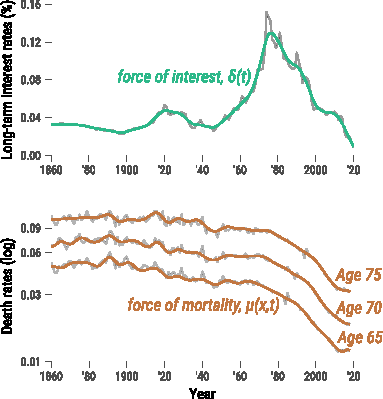
\includegraphics[width=0.5\linewidth]{Fig/deltamu}
	\caption{{Trends in interest and mortality rates calculated at ages 65, 70 and 75. Males, 1860-2018.}}
	\label{fig:Fig1}
\end{figure}


 \begin{figure}[!ht]
	\centering
	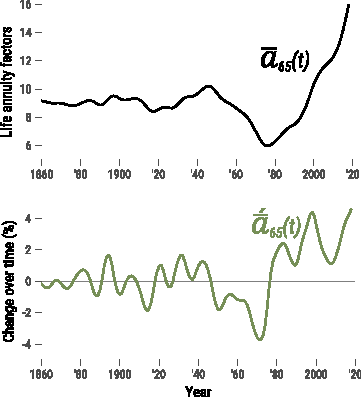
\includegraphics[width=0.5\linewidth]{Fig/axm}
	\caption{{Trends in life annuity factors and relative change in $\bar{a}_x(t)$ calculated at age 65. Males, 1860-2018.}}
	\label{fig:Fig2}
\end{figure}

\begin{figure}[!ht]
	\centering
	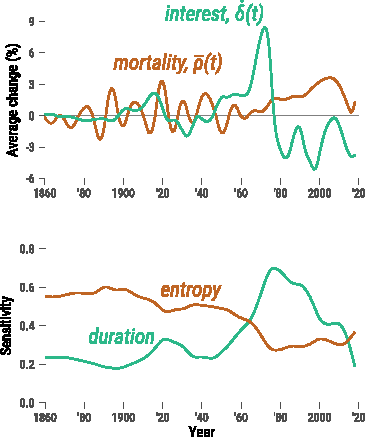
\includegraphics[width=0.5\linewidth]{Fig/IntMort}
	\caption{{Upper panel shows the average mortality improvement ($\bar{\rho}(t)$), and change in interest rates ($\dot{\delta}(t)$). Lower panel depicts the entropy ($H$) and modified duration ($D$). Males at age 65, 1860-2018.}}
	\label{fig:Fig3}
\end{figure}


\begin{figure}[!ht]
	\centering
	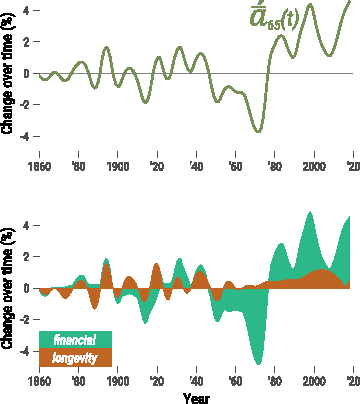
\includegraphics[width=0.5\linewidth]{Fig/DescSingle}
	\caption{{Decomposition of changes over time in life annuity factors calculated at ages 65. Males, 1860-2018.}}
	\label{fig:Fig4}
\end{figure}



\begin{figure}[!ht]
	\centering
	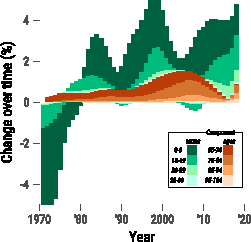
\includegraphics[width=0.4\linewidth]{Fig/DescAge}
	\caption{{Age and term attributions to changes over time in life annuity factors calculated at ages 65. Males, 1970-2018.}}
	\label{fig:Fig5}
\end{figure}


\begin{figure}[!ht]
	\centering
	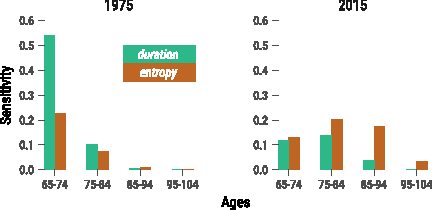
\includegraphics[width=0.7\linewidth]{Fig/AttributionDH}
	\caption{{Entropy and duration by age groups. Males, 1975 and 2015.}}
	\label{fig:Fig6}
\end{figure}

\begin{figure}[!ht]
	\centering
	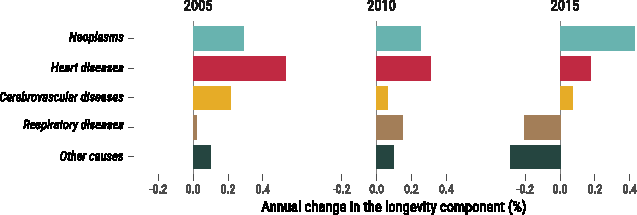
\includegraphics[width=1\linewidth]{Fig/DescCod}
	\caption{{Causes of death contributions to the changes in the longevity component. Males, 2005, 2010 and 2015.}}
	\label{fig:Fig7}
\end{figure}


\FloatBarrier
\newpage
\appendix
\section{Appendix}

\subsection{Entropy with constant changes in $\mu(x+s,t)$}\label{sec:EntropyConst}

To measure constant changes we make $\mu(s,t)+\gamma$, then

\begin{equation}\label{eq:EntropyConst1}
\begin{split}
\bar{a}_{x}(t) &= \int_0^\infty{v}(s,t) e^{-\int_{0}^{s} [\mu(x+y,t)+\gamma]dy}ds \\
&= \int_0^\infty {v}(s,t)e^{-\int_{0}^{s} \mu(x+y,t)dy} e^{-\gamma s}ds \\
&= \int_0^\infty {v}(s,t){}_sp_x(t) e^{-\gamma s}ds \\
\end{split}
\end{equation}

We expand $e^{-\gamma s}$ to $1-\gamma s+\frac{\gamma^2}{2} s^{2} +...$, so that


\begin{equation}\label{eq:EntropyConst2}
\begin{split}
\bar{a}_{x}(t) &= \int_0^\infty {}_sp_x(t) {v}(s,t)[1-\gamma s+\frac{\gamma^2}{2} s^{2} +...]ds
\end{split}
\end{equation}

We take the derivative $\bar{a}_{x}(t)$ with respect to $\gamma$ and evaluate $\gamma=0$


\begin{equation}\label{eq:EntropyConst3}
\begin{split}
{H}^{c}_x(t)&=\frac{1}{\bar{a}_x(t)}\frac{\partial \bar{a}_x(t)}{\partial \gamma} \bigg\rvert_{\gamma=0}\\
&= -\frac{\int_0^\infty s {}_sp_x(t) {v}(s,t)ds}{\bar{a}_x(t)} \\
&= \frac{{h}^{c}_x(t)}{\bar{a}_x(t)},
\end{split}
\end{equation}

where ${h}^{c}_x(t)=-\int_0^\infty s {}_sp_x(t) {v}(s,t)ds$



\subsection{Alternative expression for ${H}^{p}_{x}(t)$}\label{sec:EntropyAlt}

\begin{equation} \label{eq:EntropyAnnuityA1}
\begin{split}
{H}^{p}_{x}(t) &= -\frac{ \int_{0}^{\infty}{}_sp_x(t)\ln[{}_sp_x(t)] e^{-\int_{0}^{s}\delta(y,t)dy} ds}{\int_0^\infty {}_sp_x(t) e^{-\int_{0}^{s}\delta(y,t)dy} ds}\\
&= \frac{\int_0^\infty {}_sp_x(t) {v}(s,t) \int_0^s \mu(x+y,t) dy\,ds}{\bar{a}_x(t)}\\
&= \frac{\int_0^\infty  \mu(x+s,t) \int_s^\infty {}_yp_x(t) {v}(y,t)  dy\,ds}{\bar{a}_x(t)}\\
&= \frac{\int_0^\infty  \mu(x+s,t)  {}_sp_x(t) {v}(s,t) \int_s^\infty \frac{ {}_yp_x(t) {v}(y,t)}{ {}_sp_x(t) {v}(s,t)}  dy\,ds}{\bar{a}_x(t)}\\
&=  \frac{\int_0^\infty \mu(x+s,t)   {}_sp_x(t) {v}(s,t) \bar{a}_{x+s}(t) ds}{\bar{a}_x(t)} \\
&=  \frac{\int_0^\infty \mu(x+s,t)  {}_s|\bar{a}_x(t) ds}{\bar{a}_x(t)} \\
&=  \frac{{h}^{p}_{x}(t)}{\bar{a}_x(t)}, \\
\end{split}
\end{equation}

where ${h}^{p}_{x}(t)=\int_0^\infty \mu(x+s,t)   {}_s|\bar{a}_x(t) ds$.



\subsection{Duration with constant changes in $\delta(s,t)$}\label{sec:DurConst}

To measure constant changes we make $\delta(s,t)+\gamma$, then

\begin{equation}\label{eq:DurationConst1}
\begin{split}
\bar{a}_{x}(t) &= \int_0^\infty {}_sp_x(t) e^{- \int_{0}^{s} [\delta(y,t)+\gamma]dy}ds \\
&= \int_0^\infty {}_sp_x(t) e^{- \int_{0}^{s}\delta(y,t)dy}e^{-\gamma s}ds \\
&= \int_0^\infty {}_sp_x(t) {v}(s,t)e^{-\gamma s}ds
\end{split}
\end{equation}

We expand $e^{-\gamma s}$ to $1-\gamma s+\frac{\gamma^2}{2} s^{2} +...$, so that


\begin{equation}\label{eq:DurationConst1}
\begin{split}
\bar{a}_{x}(t) &= \int_0^\infty {}_sp_x(t) {v}(s,t)[1-\gamma s+\frac{\gamma^2}{2} s^{2} +...]ds
\end{split}
\end{equation}

We take the derivative $\bar{a}_{x}(t)$ with respect to $\gamma$ and evaluate $\gamma=0$


\begin{equation}\label{eq:DurationConst2}
\begin{split}
{D}^{c}_x(t)&=-\frac{1}{\bar{a}_x(t)}\frac{\partial \bar{a}_x(t)}{\partial \gamma} \bigg\rvert_{\gamma=0}\\
              &= \frac{\int_0^\infty s {}_sp_x(t) {v}(s,t)ds}{\bar{a}_x(t)} \\
              &= \frac{{d}^{c}_x(t)}{\bar{a}_x(t)},
\end{split}
\end{equation}

where ${d}^{c}_x(t)=\int_0^\infty s {}_sp_x(t) {v}(s,t)ds$



\subsection{Duration with proportional changes in $\delta(s,t)$} \label{sec:DurProp}

To calculate duration with proportional changes in $\delta(s,t)$, we assume that $\gamma$ is a small number such that $\delta(s,t)(1+\gamma)$ and  ${v}(s,t)=e^{-\int_0^{s}  \delta(y,t)(1+\gamma)dy}$.


\begin{equation}\label{eq:DurationProp1}
\begin{split}
\bar{a} _x(t) &= \int_0^\infty {}_sp_x(t) e^{-\int_0^{s}\delta(y,t)(1+\gamma)dy}ds \\
&= \int_0^\infty {}_sp_x(t) e^{-\int_0^{s}\delta(y,t)dy}e^{-\int_0^{s}\delta(y,t)\gamma dy}ds \\
&= \int_0^\infty {}_sp_x(t) v(s,t)v(s,t)^{\gamma}ds \\
\end{split}
\end{equation}


We expand $v(s,t)^{\gamma}$ to $1+\ln(v(s,t)) \gamma+{\ln(v(s,t))}^2 \frac{\gamma^2}{2}+...$, so that


\begin{equation}\label{eq:DurationProp2}
\begin{split}
\bar{a}_x(t) &= \int_0^\infty {}_sp_x(t) s(y,t)[1+\ln(v(s,t)) \gamma+{\ln(v(s,t))}^2 \frac{\gamma^2}{2}+...]ds\\
\end{split}
\end{equation}


To calculate the duration ${D}^{p}_{x}(t)$ we take the derivate of the expression above with respect to $\gamma$ and make $\gamma=0$

\begin{equation}\label{eq:DurationProp3}
\begin{split}
{D}^{p}_{x}(t)&=-\frac{1}{\bar{a}_x(t)}\frac{\partial \bar{a}_x(t)}{\partial \gamma} \bigg\rvert_{\gamma=0} \\
&= -\frac{\int_0^\infty {}_sp_x(t) v(s,t) \ln(v(s,t))ds}{\bar{a}_x(t)} \\
\end{split}
\end{equation}


Equation \ref{eq:DurationProp3} can be re-expressed as 


\begin{equation}\label{eq:DurationProp4}
\begin{split}
{D}^{p}_{x}(t) &= -\frac{\int_0^\infty {}_sp_x(t) v(s,t) \ln(v(s,t))ds}{\bar{a}_x(t)}\\
&= \frac{\int_0^\infty {}_sp_x(t) v(s,t) \int_0^{s} \delta(y,t)dy ds }{\bar{a}_x(t)}\\
&= \frac{\int_0^\infty \delta(s,t)  \int_{s}^{\infty} {}_{y}p_x(t) v(y,t)dy ds }{\bar{a}_x(t)}\\
&= \frac{\int_0^\infty \delta(s,t) {}_sp_x(t) v(s,t) \bar{a}_{x+s}(t)  ds }{\bar{a}_x(t)}\\
&= \frac{\int_0^\infty \delta(s,t) {}_s|\bar{a}_x(t) ds}{\bar{a}_x(t)} \\
&= \frac{{d}^{p}_{x}(t)}{\bar{a}_x(t)}.
\end{split}
\end{equation}



where ${d}^{p}_{x}(t)=\int_0^\infty \delta(s,t) {}_s|\bar{a}_x(t) ds$.





\end{document}
